\chapter{Introduksjon}
\label{chp:introduksjon}

Denne masteroppgaven omhandler bruken av pasientsignalsystemet ved St. Olavs Hospital. Disse signalene utløses av pasienter ved behov for assistanse, og leveres til sykepleiere gjennom varsling på telefon og/eller veggpaneler. 

\noindent
Vi ønsker her å gi en introduksjon til bakgrunnen for denne forskningen og redgjøre for prosjektets hensikt, samt å presentere fosrkningsspørsmålene vi har forsåkt å besvare. Tidligere forskning på temaet vil også bli presentert. Videre i oppgaven vil vi se på teori som er relevant for forskningen og presentere forskningsmetodene vi har benyttet. Deretter vil resultatene fra observasjoner og intervjuer bli presentert og diskutert før vi oppsummerer oppgaven med en konklusjon.

\section{Bakgrunn}
En overodnet oversikt over pasientsignalsystemet, og hvordan det henger sammen er illustrert i figur \ref{fig:detteskjer}. Pasientene kan tilkalle sykepleier blandt annet ved å trekke i snoren på anropspanelet, som er montert på veggen ved sengen. Signalet varsles da via vaktromsapparatet som henger synlig på sengetunet, og via rompaneler på de rommene hvor sykepleiere er tilstedemarkert (denne markeringen gjøres ved at sykepleier trykker på den grønne knappen på rompanelet). 
Sykepleieren med primæransvar for pasienten vil ved utløst pasientsignal bli varslet på sin trådløse enhet, en Cisco IP-telefon. Dersom sykepleieren ikke har mulighet til å svare, eller velger å avvise sigalet, vil neste sykepleier bli oppringt i henhold til bemanningsplanen som settes opp, og konfigureres på PC'en på sengetunet.

\begin{figure}[H]
\centering
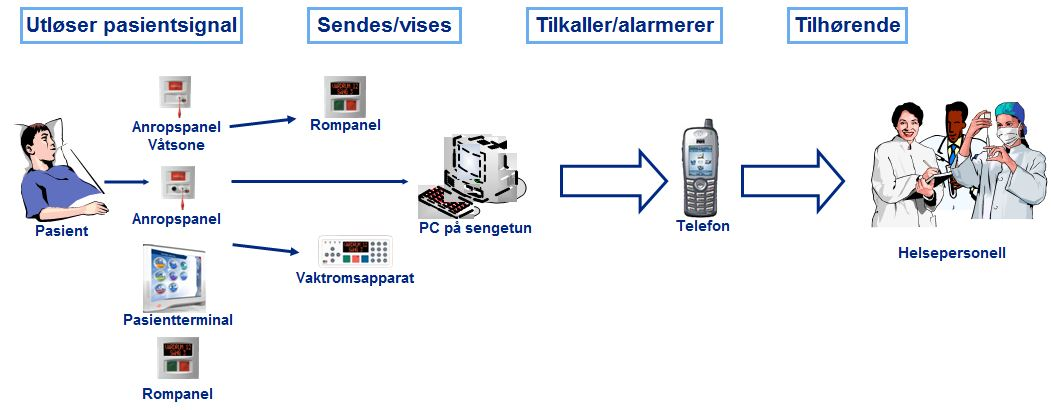
\includegraphics[scale=0.5]{alarmprosess.jpg}
\caption{Dette skjer ved utløst pasientsignal.}
\label{fig:detteskjer}
\end{figure}

\noindent
Sengepostene deles i sengetun, hvor hvert sengetun normalt har seks til åtte pasientrom. Sengetunet er en fysisk og funksjonell måte å organisere pasientrommene på, og for å sikre fleksibilitet og effektivitet ligger flere sengetun ved en sengepost etter hverandre i serie, som vist i figur \ref{fig:sengepost}. Signalsystemet kan til en viss grad konfigureres på en slik måte at sykepleiere på et sengetun kan motta pasientsignaler fra andre sengetun \citep{Aslaksen}.

\begin{figure}[H]
\centering
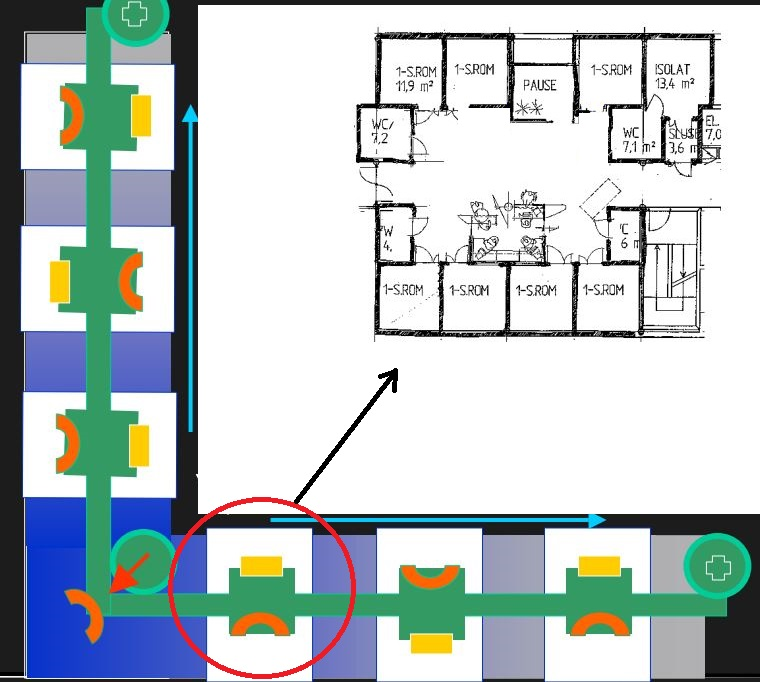
\includegraphics[scale=0.3]{sengepost.jpg}
\caption{Sengepost inndelt i sengetun \citep{Aslaksen}}
\label{fig:sengepost}
\end{figure}

\noindent
\textbf{FJERNE???} Varslingen av sykepleiere, gjør sykepleierene utsatt for eksterne avbrytelser i et allerede avbruddsdrevet miljø \citep{Klemets12}. Slike avbrudd i arbeidet kan ha både positive og negative effekter. Avbruddene kan eksempelvis gi informasjon som er nødvendig for koordinert og effektivt arbeid, og som gir bedre beslutningsgrunnlag for hvordan sykepleierne skal håndtere innkommende pasientsignaler. Slik systemet fungerer i dag er avbruddene uungåelig for å formidle denne informasjonen.
Sykepleierne vises som tilgjengelige i systemet selv når de er opptatt med oppgaver som gjør det lite ønskelig å motte pasientsignaler, som i disse tilfellene blir svært forstyrrende. \citet{KlemetsRedundancy} foreslår derfor at videre design av systemet bør tillate sykepleierene å sette seg selv som utilgjengelige. 

\section{Hensikt og foskningsspørsmål}
Motivasjonen for oppgaven har vært å kartlege sykepleiernes anvendlese av systemet, og identifisere forskjeller i bruk. Videre ønsket vi å svare på hva som kan være årsaker til at disse forskjellende har oppstått. 

\noindent
Da vi startet arbeidet med denne oppgaven var tanken at vi skulle se på hvordan systemet kunne endres for å bedre møte sykepleiernes behov. Etter første observasjonsrunde så vi imidlertid at en mer interessant vinkling ville være å se på hvordan systemet blir brukt forskjellig på de forskjellige avdelingene, og hva de bakenforliggende årsakende til dette kan være. Dette resulterte i to forskningsspørsmål:

\begin{enumerate}
\item Hvordan brukes pasientsignalsystemet ved St.Olavs hospital forskjellig i, og mellom ulike avdelinger? 
\item Hvilke faktorer kan være årsak til disse forskjellene?
\end{enumerate}

\noindent
For å besvare disse spørsmålene har vi gjennomført både observasjoner og semistrukturerte intervjuer ved tre avdelinger ved St.Olavs hospital. Dataene fra disse innsamlingene ble så analysert og valg av relevent teori ble gjort i tråd med stegvis-deduktiv induktiv metode. Forskningsmetodene vi har anvendt er nærmere beskrevet i kapittel \ref{chp:metode}.

\section{Tidligere arbeid}